\chapter{Diseño de la red}

\section{Vista general}

La solución utiliza una VPC no predeterminada para que cada ruta y asociación sea deliberada. El bloque \code{10.10.0.0/24} pertenece al espacio privado de RFC 1918 y contiene 256 direcciones. Cinco bloques se materializan como subredes; el sexto se conserva como reserva lógica. Todas las subredes del prototipo se colocan en la primera zona disponible de la región elegida. AWS establece que cada subred pertenece por completo a una zona de disponibilidad y no puede abarcar varias \cite{aws-configure-subnets}.

\begin{figure}[H]
\centering
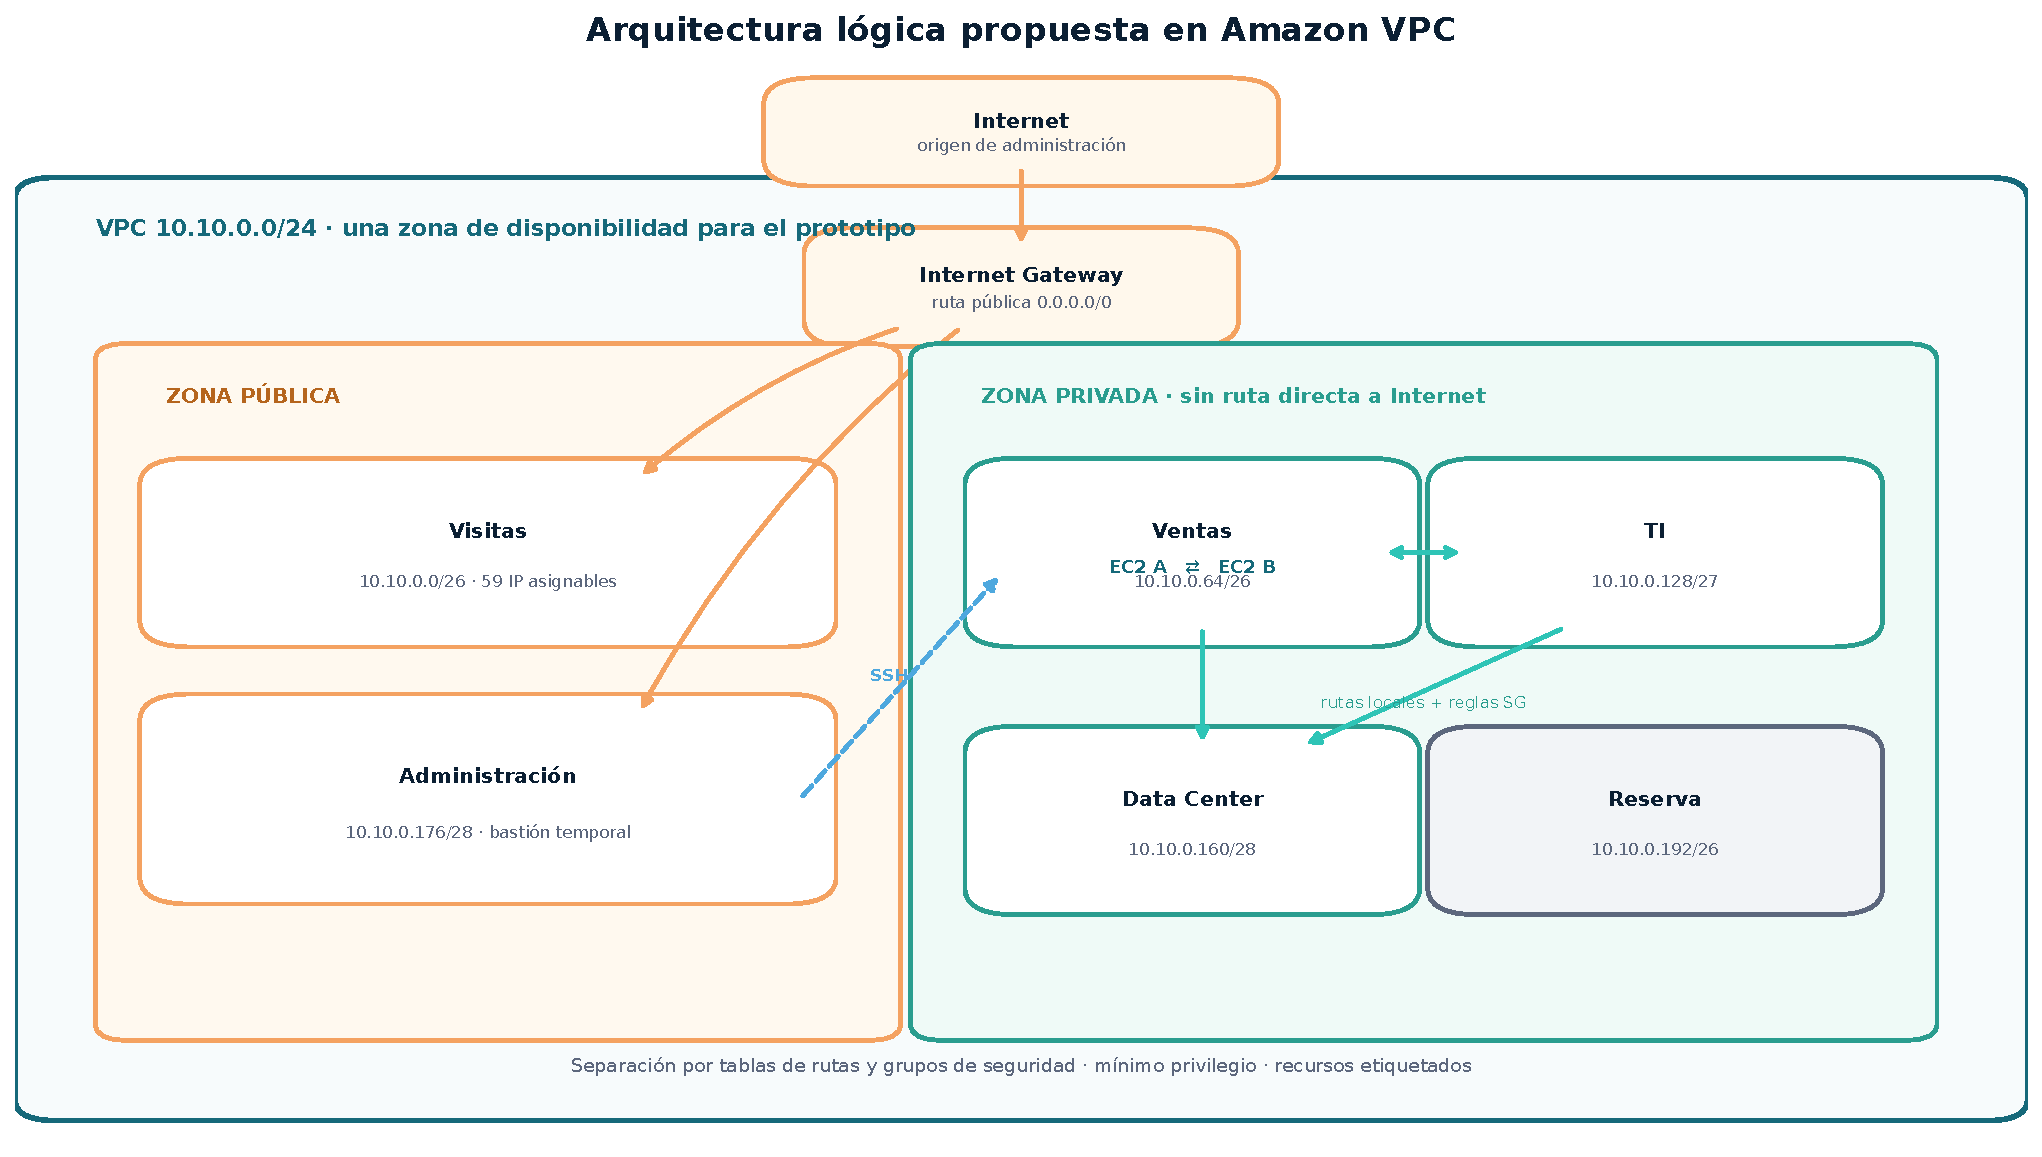
\includegraphics[width=\textwidth]{arquitectura-vpc.pdf}
\caption{Arquitectura lógica de la VPC propuesta. Elaboración propia.}
\label{fig:architecture}
\end{figure}

\section{Componentes}

\subsection{VPC}

La VPC habilita resolución y nombres DNS para facilitar una evolución posterior. Su tabla principal se mantiene sin rutas públicas adicionales. Esta decisión reduce el riesgo de que una subred creada en el futuro herede accidentalmente salida directa a Internet: las asociaciones con tablas personalizadas son explícitas.

\subsection{Subredes públicas}

Visitas y Administración se asocian con \code{public-rt}, que contiene la ruta local creada por AWS y \code{0.0.0.0/0} hacia el Internet Gateway. Ninguna de las dos habilita asignación automática de IP pública. De este modo, la clasificación ``pública'' depende del enrutamiento, pero cada recurso debe solicitar de forma deliberada una dirección pública.

Administración aloja únicamente el bastión temporal. Visitas se crea para demostrar la segmentación, pero la fase no ejecuta clientes invitados. En una ampliación real, sus dispositivos podrían acceder a Internet mediante un mecanismo diseñado para ese fin, manteniendo denegado el acceso a los segmentos internos.

\subsection{Subredes privadas}

Ventas, TI y Data Center se asocian con \code{private-rt}. La tabla sólo conserva la ruta \code{local} que AWS instala para el CIDR de la VPC. No se agrega NAT Gateway ni ruta a un Internet Gateway. Por tanto, las instancias de Ventas no pueden descargar paquetes desde Internet, pero sí intercambiar tráfico privado si los grupos de seguridad lo permiten.

\subsection{Bloque de reserva}

El bloque \code{10.10.0.192/26} no se declara como subred. Reservarlo permite incorporar posteriormente otra zona de disponibilidad, servicios compartidos o expansión departamental. Mantenerlo sin asignar evita asumir prematuramente su propósito y no consume recursos de AWS.

\section{Enrutamiento}

Cada subred debe estar asociada con una tabla de rutas, de manera explícita o implícita. Una tabla puede servir a varias subredes, pero cada subred sólo puede asociarse con una tabla a la vez \cite{aws-route-tables}. El prototipo aplica las siguientes decisiones:

\begin{table}[H]
\centering
\caption{Tablas de rutas propuestas}
\begin{tabularx}{\textwidth}{p{3.2cm}p{3.1cm}p{3.3cm}Y}
\toprule
\textbf{Tabla} & \textbf{Destino} & \textbf{Objetivo} & \textbf{Asociaciones} \\
\midrule
Pública & \code{10.10.0.0/24} & \code{local} & Visitas, Administración \\
Pública & \code{0.0.0.0/0} & Internet Gateway & Visitas, Administración \\
Privada & \code{10.10.0.0/24} & \code{local} & Ventas, TI, Data Center \\
\bottomrule
\end{tabularx}
\end{table}

AWS aplica coincidencia de prefijo más largo al elegir una ruta. La ruta local \code{/24} es más específica que \code{/0}; por ello el tráfico entre direcciones internas permanece dentro de la VPC. La ruta predeterminada sólo captura destinos no incluidos en el bloque local.

\section{Flujos representativos}

\subsection{Administración hacia Ventas}

El operador se conecta al bastión por SSH desde la única IP autorizada. Desde allí establece otro túnel SSH hacia la IP privada de la instancia de Ventas. El grupo de seguridad de Ventas no acepta SSH desde un CIDR arbitrario: referencia directamente el grupo de seguridad del bastión. Si la IP pública del operador cambia, se actualiza sólo \code{admin\_cidr}.

\subsection{Ventas hacia Ventas}

Las dos instancias comparten \code{ventas-sg}. Una regla ICMP con \code{self=true} acepta eco entre interfaces vinculadas al mismo grupo. El paquete se entrega por la ruta local y nunca sale hacia Internet. Éste es el flujo utilizado para la prueba de concepto.

\subsection{Visitas hacia redes internas}

La ruta local hace técnicamente alcanzables los prefijos de la VPC en la capa de enrutamiento, pero los grupos de seguridad de las cargas internas no contienen reglas que acepten tráfico originado por Visitas. En una versión productiva se complementaría este control con Network ACL o un firewall administrado si se requiere separación sin estado en el límite de subred.

\section{Escalabilidad}

El prototipo prioriza claridad y economía, no alta disponibilidad. Para producción se recomienda utilizar el bloque de reserva o ampliar el CIDR, duplicar subredes en otra zona y separar Administración de cualquier red de usuarios. También conviene reemplazar el bastión público por mecanismos administrados de acceso y añadir registros de flujo. Estas mejoras no alteran el aprendizaje central: los segmentos conservan prefijos distintos y políticas explícitas.
